\subsection*{Data acquisition}
We recorded the calcium activity  of dense populations of neurons in the supragranular layers in primary visual cortex of anesthetized mice using fast random-access 3D scanning two-photon microscopy \cite{Stosiek:2003,Reddy:2005}.  Numerious repetitions of full-field drifting gratings (Fig. 1A and 1B) were presented to the eye contralateral to the imaged site. This technique allowed recording from a large number (150--350) of cells in a small volume of cortical tissue ($200\times200\times100$ $\mu$m$^3$) in layers 2/3 and 4. Somatic calcium signals were deconvolved using  sparse nonnegative deconvolution \cite{Vogelstein:2010} (Fig.\;1C and 1D).  The average stimulus response was subtracted to remove stimulus covariance and the sample noise covariance matrix was computed (Fig.\;1E).

\begin{figure}[htp]
\begin{center}
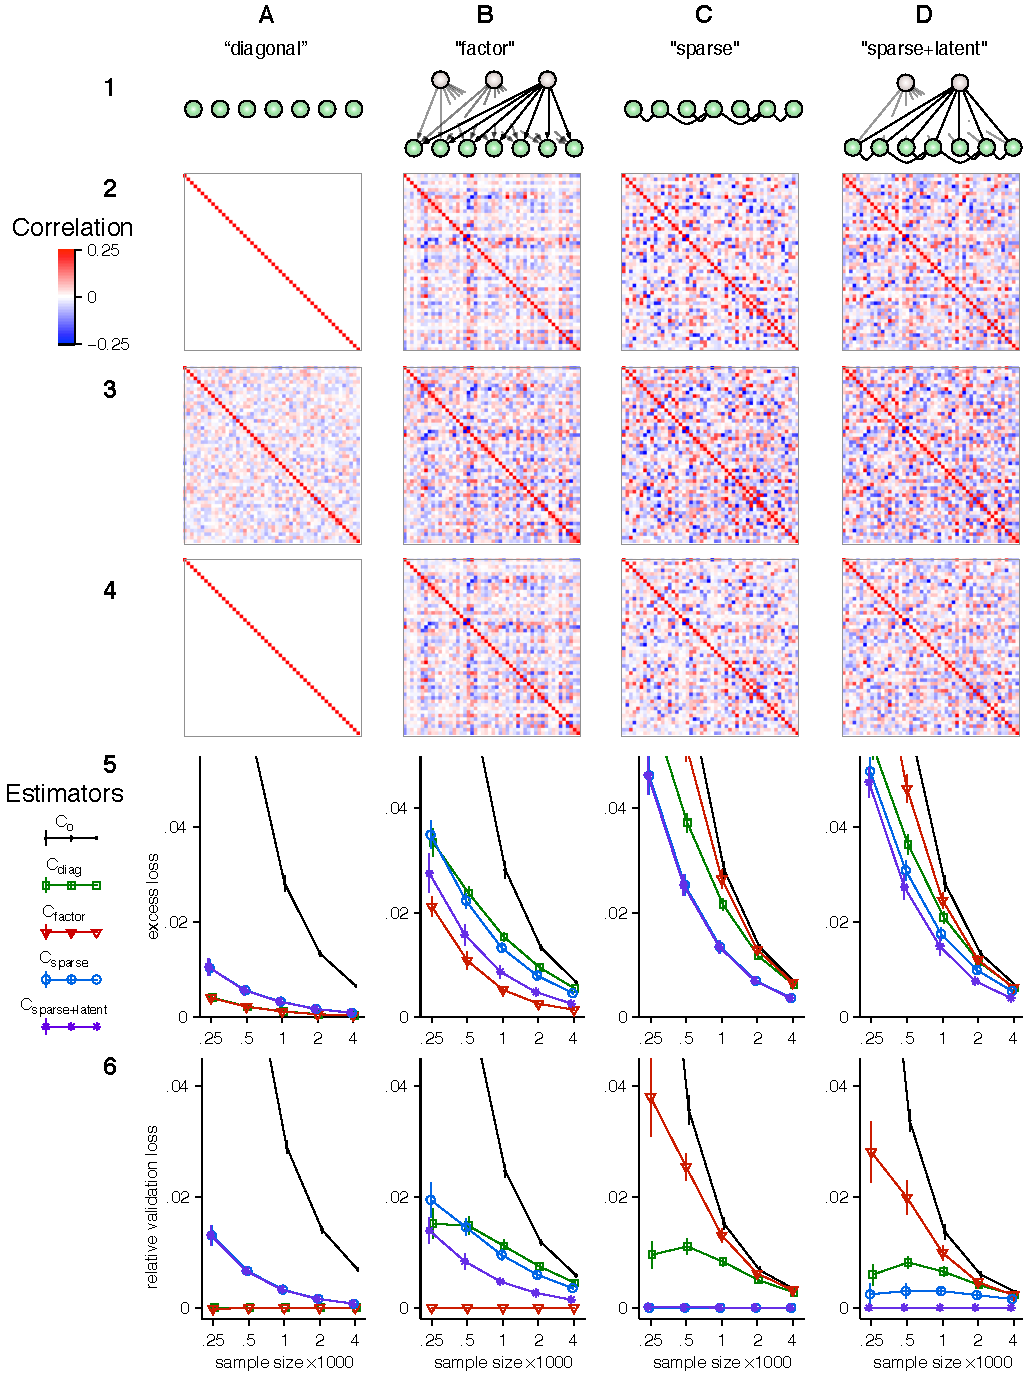
\includegraphics[width=2.5in]{figures/Figure1.pdf}
\end{center}
\caption{
{\bf Acquistion of neural population activity using two-photon fluorescence imaging of calcium signal.}  {\bf A.} Visual stimuli comprising brief (500 ms) presentatios of full-field drifting gratings separated by blank screens. {\bf B.} Two-photon fast 3D imaging of calcium signals in an awake mouse. {\bf C.} Deconvolved calcium signals. {\bf D.} The sample covariance matrix of neuronal calcium signals in 200 ms time bins. 
}
\label{Figure_label}
\end{figure}

